% ====================================================================
% VİZE RAPOR ŞABLONU – Türk Masalları Derlemesi Web Sayfası
% --------------------------------------------------------------------
% DERLEME: Overleaf'te Menu > Compiler > XeLaTeX (pdfLaTeX de çalışır).
%
% KURALLAR (şablonu kullanmadan önce okuyun):
%  1. Bölüm başlıklarını SİLMEYİN ve sırasını DEĞİŞTİRMEYİN.
%  2. [KÖŞELİ PARANTEZ] içindeki ve gri renkli açıklama metinlerini
%     kendi bilgilerinizle değiştirin; açıklama metinlerini silin.
%  3. MEBİS'e YALNIZCA bu raporun PDF'ini yükleyin.
%     ZIP ve HTML dosyası YÜKLEMEYİN. Tüm kontroller GitHub'dan yapılır.
%  4. Kapaktaki GitHub ve YouTube bağlantıları doğru ve tıklanabilir
%     olmalıdır. Teslimden önce PDF'teki bağlantılara tıklayıp deneyin.
%  5. Haftalık katkı tablosundaki görseller için resim dosyalarını
%     (hafta1.png, hafta2.png, ...) Overleaf projesine yükleyin.
%     Dosya adlarında boşluk ve Türkçe karakter kullanmayın.
%     Resim yoksa tabloda "görsel ekleyin" kutusu görünür.
%  6. Yapay zekâ kullandıysanız Bölüm 5'i doldurun.
% ====================================================================
\documentclass[12pt,a4paper]{article}

\usepackage{iftex}
\ifPDFTeX
  \usepackage[T1]{fontenc}
  \usepackage[utf8]{inputenc}
\else
  \usepackage{fontspec}
\fi
\usepackage[turkish]{babel}
\usepackage[margin=2.4cm]{geometry}
\usepackage{setspace}
\usepackage{graphicx}
\usepackage{booktabs}
\usepackage{longtable}
\usepackage{array}
\usepackage{colortbl}
\usepackage{xcolor}
\usepackage{enumitem}
\usepackage{listings}
\usepackage{amssymb}
\usepackage{caption}
\usepackage{fancyhdr}
\usepackage{hyperref}

\onehalfspacing
\setlength{\parindent}{0pt}
\setlength{\parskip}{6pt}
\setlist{itemsep=2pt, topsep=4pt}
\hypersetup{colorlinks=true, linkcolor=blue!50!black, urlcolor=blue!50!black}

\definecolor{ana}{HTML}{14325C}
\definecolor{acik}{HTML}{EEF2F8}

\lstset{basicstyle=\ttfamily\small, backgroundcolor=\color{acik},
  frame=single, rulecolor=\color{ana}, breaklines=true,
  columns=fullflexible, keepspaces=true, showstringspaces=false}

\pagestyle{fancy}
\fancyhf{}
\fancyhead[L]{[ Bir Varmış Bir Yokmuş-Türk Masalları Derlemesi Web Sayfası]}
\fancyhead[R]{Vize Raporu}
\fancyfoot[C]{\thepage}

% ---------- Yardımcı komutlar ----------
% Gri açıklama metni (silinecek yönergeler için)
\newcommand{\aciklama}[1]{{\color{gray}\itshape (#1)}}

% Haftalık tablo görseli: dosya yoksa "görsel ekleyin" kutusu çıkar
\newcommand{\haftagorsel}[1]{%
  \IfFileExists{#1}{%
    \includegraphics[width=\linewidth,height=4.2cm,keepaspectratio]{#1}%
  }{%
    \fbox{\parbox[c][2.6cm][c]{\dimexpr\linewidth-2\fboxsep-2\fboxrule\relax}{%
      \centering\small\color{gray} Ekran görüntüsü / görsel ekleyin\\ \texttt{#1}}}%
  }%
}
% Haftalık katılım kutuları (işaretlemek için $\square$ yerine $\boxtimes$ yazın)
\newcommand{\katilimkutulari}{\par\vspace{3pt}\small $\square$ Ders içinde katılım sergiledim\par $\square$ Telafi yaptım}

% Ek görsel: dosya yoksa hiçbir şey göstermez
\newcommand{\haftaek}[1]{%
  \IfFileExists{#1}{\\[4pt]\includegraphics[width=\linewidth,height=4.2cm,keepaspectratio]{#1}}{}%
}

% ---------- Kapak bilgileri ----------
\newcommand{\universite}{[ÜNİVERSİTE / BÖLÜM]}
\newcommand{\dersadi}{[DERS ADI]}
\newcommand{\hocaadi}{[ÖĞRETİM ÜYESİ]}
\newcommand{\ogrenciadi}{[AD SOYAD]}
\newcommand{\ogrencino}{[ÖĞRENCİ NUMARASI]}
\newcommand{\projeadi}{[PROJE ADI]}
% Bağlantıları tam adres olarak yazın (https:// ile başlayarak)
\newcommand{\githublink}{\url{https://github.com/KULLANICI-ADI/DEPO-ADI}}
\newcommand{\youtubelink}{\url{https://www.youtube.com/watch?v=VIDEO-KIMLIGI}}

\begin{document}

% ====================================================================
% KAPAK
% ====================================================================
\begin{titlepage}
\centering
\vspace*{1cm}
{\large \ İstanbul Medipol Üniversitesi \par}
\vspace{1.8cm}
{\Huge\bfseries\color{ana} \ Bir Varmış Bir Yokmuş \par}
\vspace{0.4cm}
{\Large Türk Masalları Derlemesi Web Sayfası \par}
{\large Vize Raporu \par}
\vspace{1.8cm}
{\large \textbf{Ders:} \ Programlamaya Giriş \par}
{\large \textbf{Öğretim Üyesi:} \ Meral Şentürk \par}
\vspace{1.2cm}
{\large \textbf{Hazırlayan:} \ Elif Salbaz \par}
{\large \textbf{Öğrenci No:} \ 86250013 \par}
\vspace{1.8cm}
\fbox{\parbox{0.88\linewidth}{\centering\vspace{6pt}
{\large\bfseries Proje Bağlantıları}\\[8pt]
\textbf{GitHub deposu:}https://github.com/salbazelif/Vize-devi.git\\[8pt]
\textbf{YouTube sunum videosu:} https://youtu.be/veWg5lkkeus
\vspace{6pt}}}
\vfill
{\large \today \par}
\end{titlepage}

\tableofcontents
\newpage

% ====================================================================
\section{Giriş}
% ====================================================================
 Bu  projenin amacı, Türk halk masallarının kısa özetlerini bir araya getirerek kullanıcıların masalları kolayca keşfedebileceği bir web sayfası oluşturmaktır. Projemde Keloğlan ve Dev, Altın Saçlı Kız ve Zümrüdüanka Kuşu gibi toplam 10 masala yer vererek 8–12 masal şartını karşıladım. Kullanıcıların istedikleri masala ulaşabilmesi için masal kartları, arama alanı ve özet görüntüleme işlevleri oluşturdum. Masal atmosferini desteklemek ve okumayı kolaylaştırmak amacıyla pastel renkler, krem zemin ve Georgia yazı tipini tercih ettim. Sayfanın tamamını tek bir HTML dosyasında hazırlayarak CSS kodlarını dosyanın içindeki `<style>`, JavaScript kodlarını ise `<script>` etiketi altında topladım. Böylece tek HTML dosyası, içsel CSS ve içsel JavaScript gereksinimlerini karşıladım. Bu raporda masalların seçimi ve kaynakları, tasarım kararları, kodların çalışma mantığı, yapay zekâ kullanımı ve ders içi haftalık katkılarım yer almaktadır..

\subsection{Proje Özeti}
Proje, 10 farklı masalın kısa özetlerini bir araya getiren bir web sayfasıdır. Ana sayfada kullanıcıları masal dünyasına davet eden bir karşılama alanı ve site hakkında kısa bir açıklama bulunmaktadır. Masal kitaplığında her masal, başlığının ve okuma butonunun yer aldığı renkli bir kartla sunulmaktadır. Kullanıcılar bu kartlardan istedikleri masalı seçerek özetini ayrı bir alanda okuyabilmektedir. Arama kutusu, masal adlarına göre filtreleme yaparak istenen içeriğe ulaşmayı kolaylaştırmaktadır. Menü ve geri dönüş butonları sayesinde ana sayfa, kitaplık ve masal özetleri arasında geçiş yapılabilmektedir. Pastel renkler, Georgia yazı tipi ve farklı ekran boyutlarına uyum sağlayan düzenle sade ve okunabilir bir arayüz oluşturulmuştur.

\subsection{Gereksinimlerin Karşılanması}
\begin{center}
\rowcolors{2}{acik}{white}
\begin{tabular}{@{}p{8.2cm}c@{}}
\toprule
\rowcolor{ana}\textcolor{white}{\textbf{Gereksinim}} & \textcolor{white}{\textbf{Durum}} \\
\midrule
Masal sayısı 8--12 arasında (10 masal)         & $\boxtimes$ \\
Tek HTML dosyası                                    & $\boxtimes$ \\
Stil kodları içsel (\texttt{<style>} içinde)        & $\boxtimes$ \\
Betik kodları içsel (\texttt{<script>} içinde)      & $\boxtimes$ \\
İnternetsiz açılıp çalışıyor                        & $\boxtimes$ \\
JavaScript sayfada anlamlı bir işlev görüyor        & $\boxtimes$ \\
Masal metinleri kendi cümlelerimle yazıldı          & $\square$ \\
Sayfa telefonda da düzgün görünüyor                 & $\boxtimes$ \\
\bottomrule
\end{tabular}
\end{center}
% ====================================================================
\section{Masalların Seçimi}
% ====================================================================
\begin{longtable}{@{}cp{4cm}p{3cm}p{5.4cm}@{}}
\toprule
\textbf{No} & \textbf{Masal} & \textbf{Tür} & \textbf{Seçilme nedeni} \\
\midrule
\endhead
1 & Keloğlan ve Dev & [Olağanüstü masal] & Tanıdığım Keloğlan karakterine yer vermek ve zekâyla sorun çözme temasını göstermek için seçtim.\\
2 & Altın Saçlı Kız & Olağanüstü masal & Araştırırken dikkatimi çektiği ve sabır ile kararlılık temalarını içerdiği için seçtim. \\
3 & Aslan Padişah ile Fare & Hayvan masalı & Hayvan karakterler üzerinden yardımlaşmayı anlatması nedeniyle seçtim. \\
4  & Tombul Gözleme & Zincirleme masal & Tekrarlanan karşılaşmaları ve eğlenceli anlatımıyla çeşitlilik sağlaması için seçtim. \\
5 & Altın Top & Olağanüstü masal & [Verilen sözün tutulması temasını işlemesi nedeniyle seçtim. \\
6 & Üç Turunçlar & Olağanüstü masal & Sihirli turunçlar ve yolculuk gibi fantastik unsurları ilgimi çektiği için seçtim. \\
7 & Nardaniye Hanım & Olağanüstü masal & [İyilik, kötülük ve kıskançlık temalarına yer vermesi nedeniyle seçtim. \\
8 & Zümrüdüanka Kuşu & Olağanüstü masal & Fantastik kuş figürü ve maceralı olaylarıyla dikkatimi çektiği için seçtim. \\
9 & Tuz Kadar Sevgi & Gerçekçi masal & Sevginin değerini günlük hayattan bir örnekle anlatması nedeniyle seçtim. \\
10 & Kabak Gelin & Olağanüstü masal &  Farklı kahramanı ve dönüşüm unsurlarıyla derlemeyi çeşitlendirmek için seçtim. \\
\bottomrule
\end{longtable}

% ====================================================================
\section{Tasarım Kararları}
% ====================================================================
Web sayfasında, kullanıcıların masal özetlerine kolayca ulaşabileceği sade bir düzen oluşturulmuştur. Masallar kartlar hâlinde sunulmuş, “Özeti Oku” butonları ve arama alanıyla içeriklere erişim kolaylaştırılmıştır. Özetlerin ayrı bir alanda gösterilmesiyle okuyucunun metne odaklanması amaçlanmıştır.

Krem zemin ve koyu bordo yazılarla okunabilirlik desteklenmiş, kitap sayfalarını çağrıştıran Georgia yazı tipi tercih edilmiştir. Satır aralıkları ve boşluklar rahat okumaya uygun düzenlenmiştir. Menü ve geri dönüş butonlarıyla kolay gezinme sağlanırken ekran genişliğine göre değişen kart düzeniyle telefon ve bilgisayar kullanımına uyum hedeflenmiştir.

\subsection{Konuya Uygunluk}
“Bir Varmış Bir Yokmuş” sitesinde pastel pembe, lila ve krem tonları, masalların hayal dünyasına uygun sıcak bir atmosfer oluşturmak için seçilmiştir. Krem zemin üzerindeki koyu bordo yazılarla okunabilirlik desteklenmiştir. Georgia yazı tipi, geleneksel masal kitaplarını çağrıştırdığı için tercih edilmiştir. Ana sayfadaki şato ve doğa manzarası, masallarda karşılaşılan uzak diyarları ve olağanüstü mekânları hatırlatarak sitenin temasını tamamlamaktadır.

\subsection{Renk Paleti ve Yazı Tipi}
\begin{center}
\rowcolors{2}{acik}{white}
\begin{tabular}{@{}llp{6.4cm}@{}}
\toprule
\rowcolor{ana}\textcolor{white}{\textbf{Ad}} & \textcolor{white}{\textbf{Kod}} & \textcolor{white}{\textbf{Nerede / neden kullandınız?}} \\
\midrule
 \relax Pastel pembe & \texttt {[\#D6A5B3]}   &  Üst ve alt bilgi alanlarında sıcak, masalsı bir atmosfer oluşturmak için kullanılmıştır. \\
\relax Krem & \texttt {[\#FFF8F2]}  & Ana zeminde, koyu yazıların rahat okunmasını sağlamak için kullanılmıştır.\\
\relax Koyu bordo & \texttt {[\#783B50]}  & Metinlerde ve menü bağlantılarında açık zemin üzerinde belirginlik sağlamak için kullanılmıştır.\\
\relax Açık lila & \texttt {[\#E8DDF5]}  & Karşılama alanını vurgulamak ve masalsı atmosferi desteklemek için kullanılmıştır.\\
\relax Açık pembe & \texttt {[\#F9E9ED]}  & Menü, masal kartları ve özet alanını Nana zeminden ayırmak için kullanılmıştır. \\ 
\relax Georgia & -- & Başlık ve metinlerde, geleneksel masal kitaplarını çağrıştıran görünümü nedeniyle tercih edilmiştir. \\
\bottomrule
\end{tabular}
\end{center}

\subsection{Okunabilirlik, Gezinme ve Duyarlı Tasarım}
\begin{itemize}
  \item \textbf{Okunabilirlik:} Açık krem zemin üzerinde koyu renkli metinler kullanılarak yazıların kolay okunması sağlanmıştır. Georgia yazı tipi, belirgin başlıklar ve uygun satır aralıklarıyla rahat bir okuma düzeni oluşturulmuştur.
  \item \textbf{Gezinme:} Kullanıcılar ana sayfadaki masal kartları aracılığıyla istedikleri masala ulaşabilmektedir. Menü bağlantıları ve geri dönüş butonları sayesinde sayfalar arasında kolayca gezinebilmektedir.
  \item \textbf{Duyarlı tasarım:} Web sitesi, bilgisayar ve telefon ekranlarına uyum sağlayacak şekilde tasarlanmıştır. Bilgisayarda geniş bir yerleşim kullanılırken telefon ekranında içerikler ekran genişliğine göre yeniden düzenlenmektedir.
  \item \textbf{Tutarlılık:} Sitenin bütün sayfalarında aynı renk paleti, yazı tipi ve başlık düzeni kullanılmıştır. Boşluklar, menüler ve masal kartları arasında görsel bütünlük sağlanarak tutarlı bir tasarım oluşturulmuştur.
\end{itemize}

\subsection{Ekran Görüntüleri}
\begin{figure}[h]
  \centering
  \resizebox{0.65\textwidth}{!}{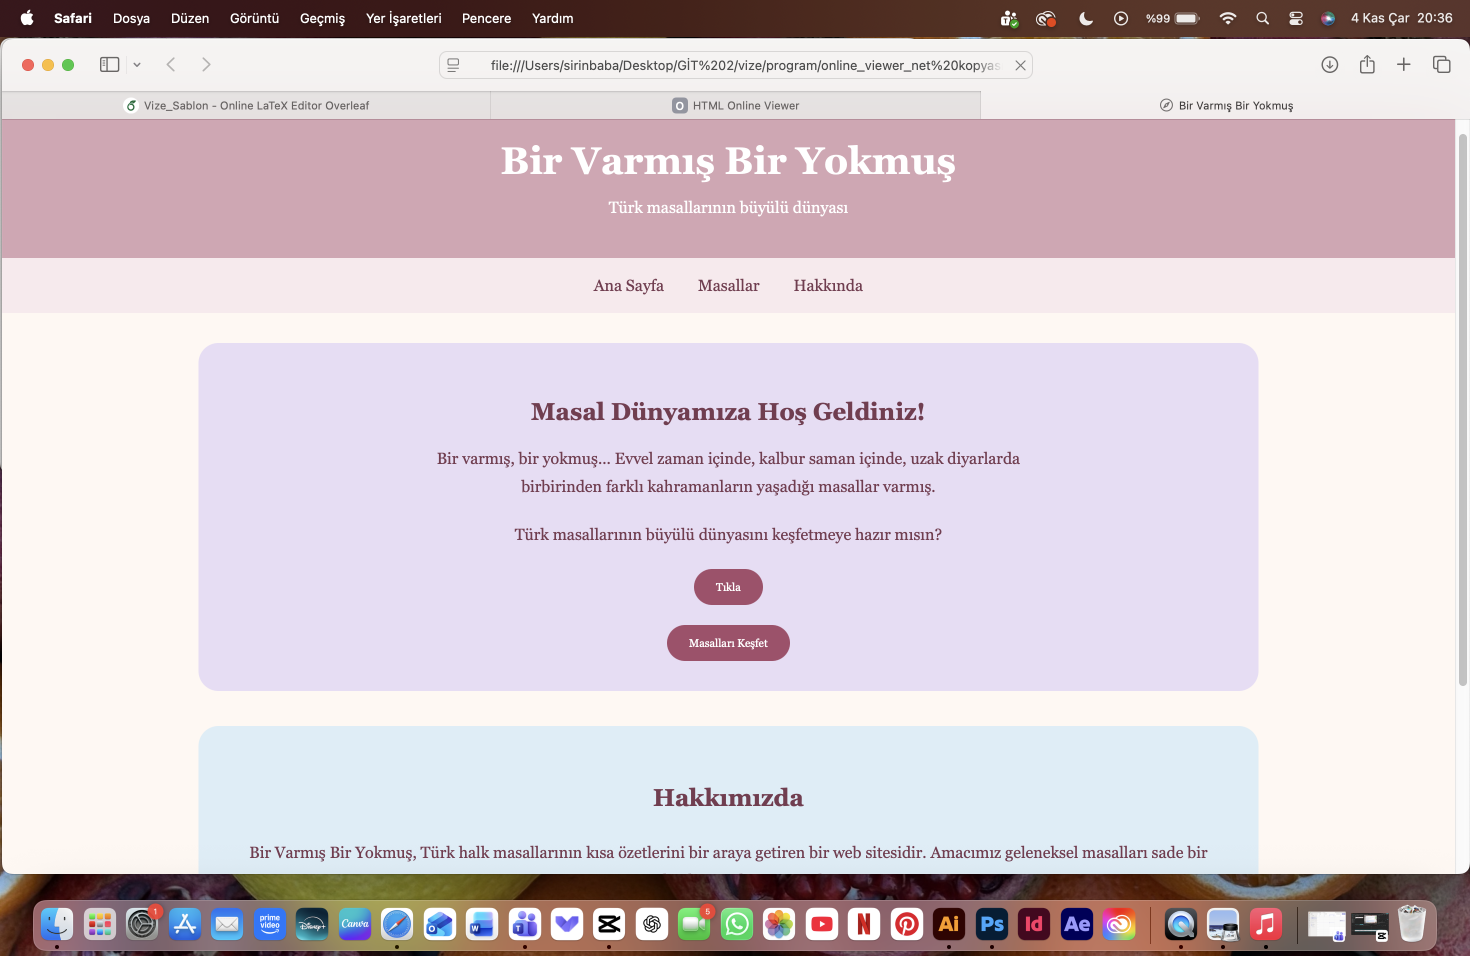
\includegraphics{ekran-masaustu.png}}
  \caption{Sayfanın bilgisayar görünümü}
\end{figure}

\begin{figure}[h]
  \centering
  \resizebox{0.20\textwidth}{!}{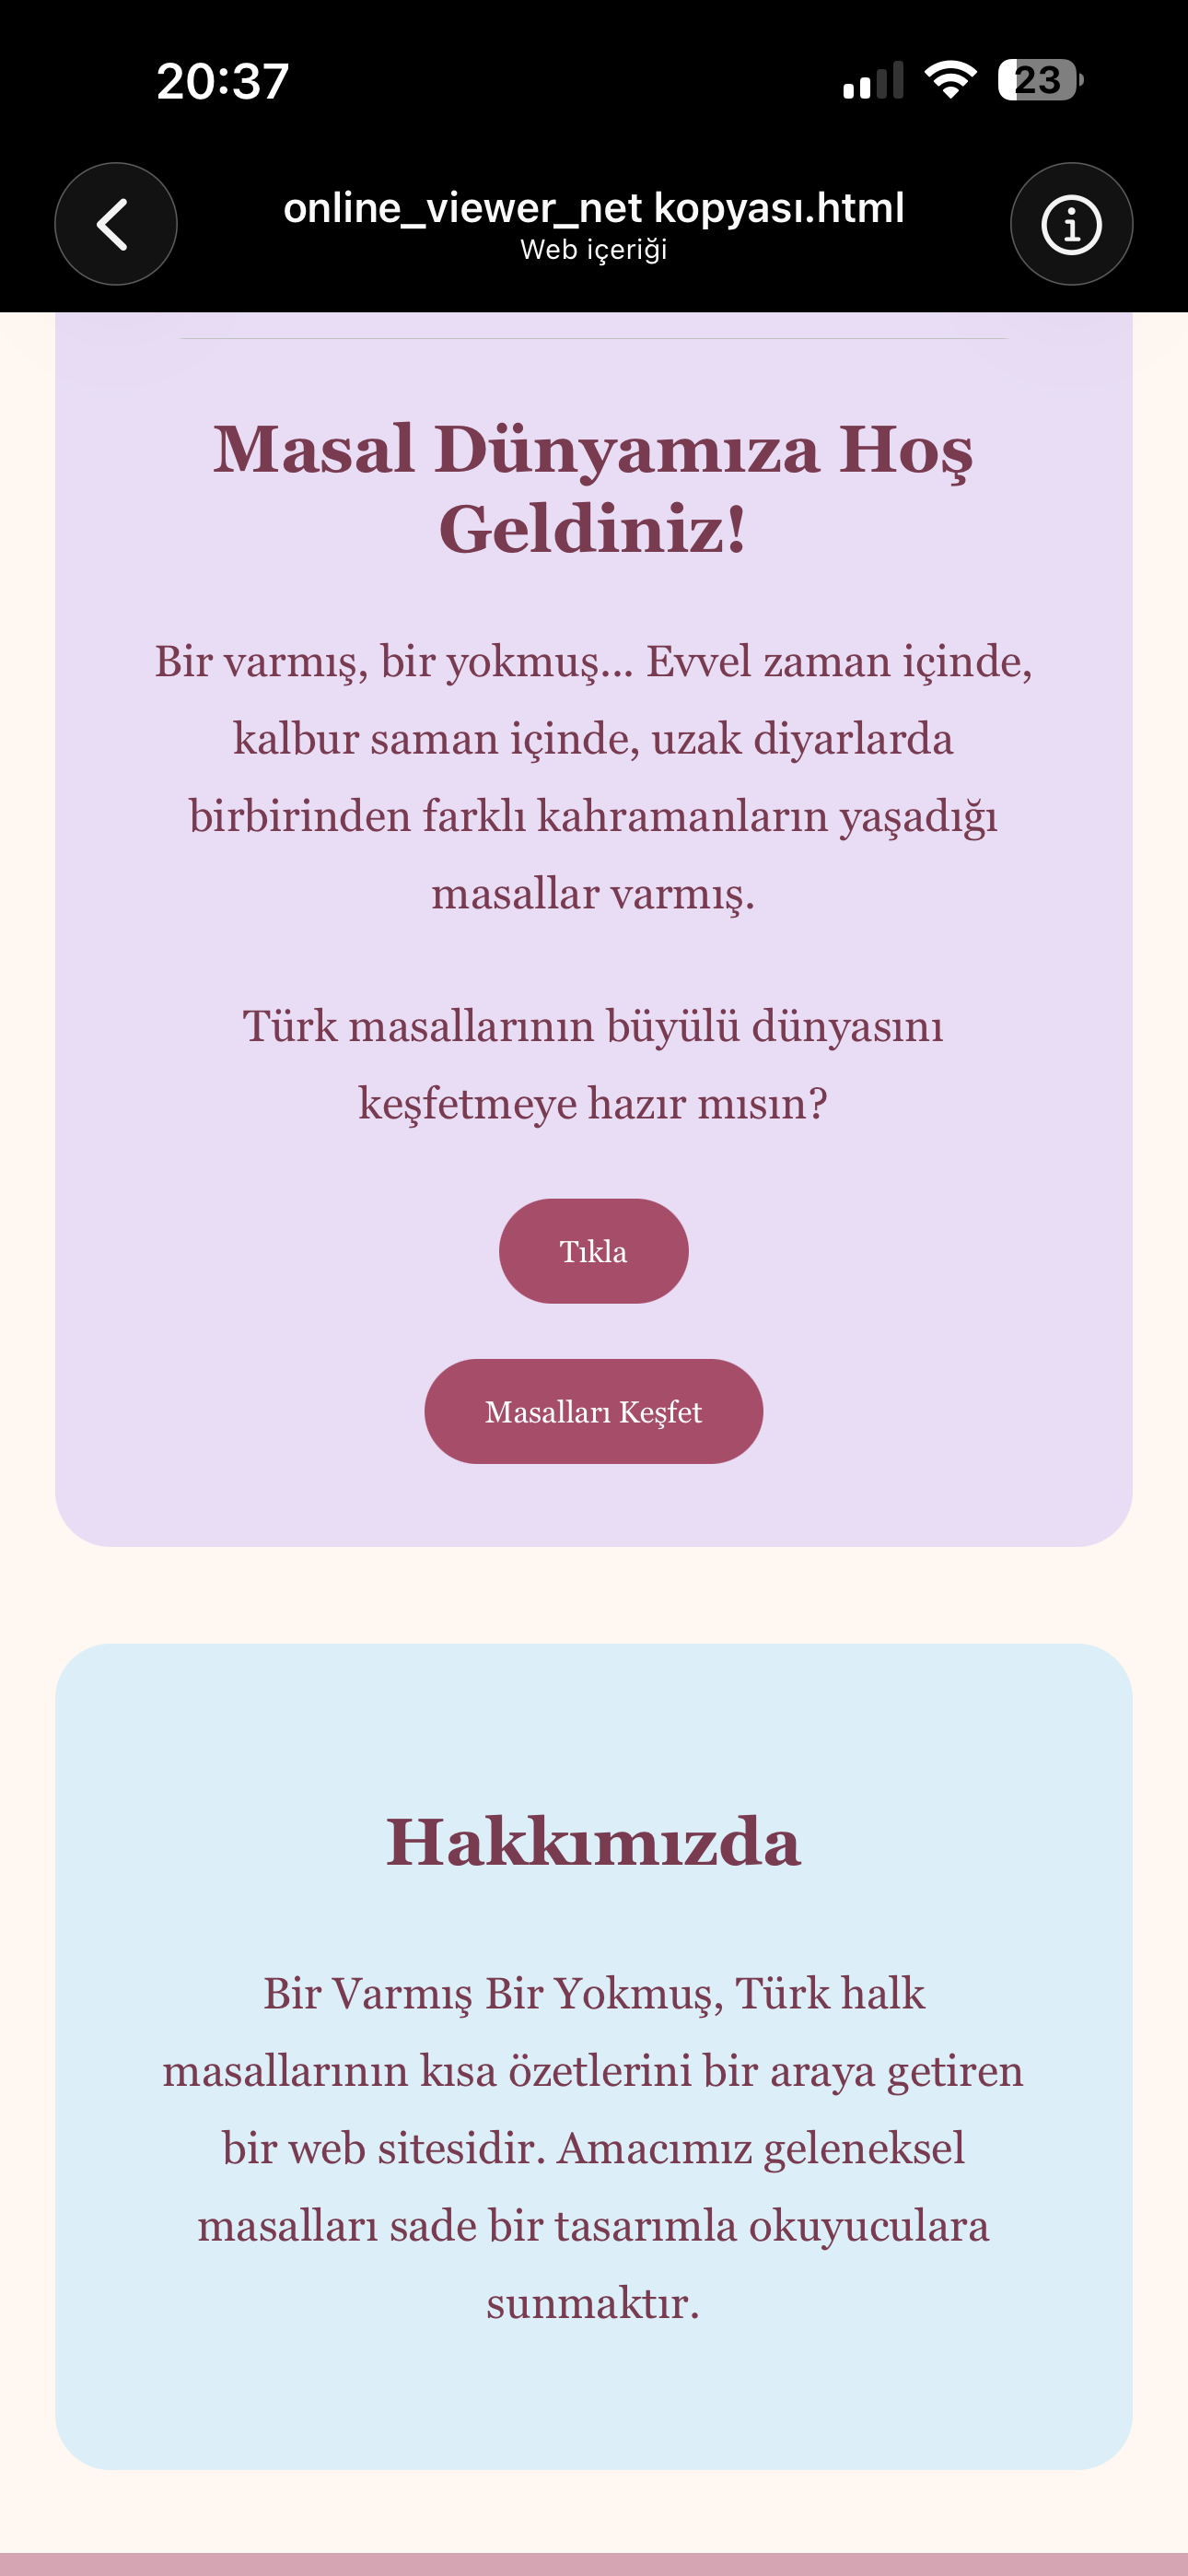
\includegraphics{ekran-mobil.png}}
  \caption{Sayfanın telefon görünümü}
\end{figure}
% ====================================================================
\section{Gerçekleştirme}
% ====================================================================
 Bir Varmış Bir Yokmuş” adlı web sitesi, kullanıcıların Türk masallarına kolayca ulaşabilmesi ve okuyabilmesi amacıyla hazırlanmıştır. Sitenin yapısında HTML, görsel düzeninde ise CSS kullanılmıştır. 
HTML ile başlıklar, menü bağlantıları, masal kartları ve metin alanları oluşturulmuştur. CSS ile bu bölümlerin renkleri, yazı tipleri, boyutları ve sayfa üzerindeki yerleşimleri düzenlenmiştir.
Ana sayfada bulunan masal kartları sayesinde kullanıcılar okumak istedikleri masalı seçebilmektedir. Masal sayfalarında metinler düzenli bir şekilde sunulmuş, gezinme bağlantılarıyla sayfalar arasında geçiş kolaylaştırılmıştır.
Ayrıca farklı ekran boyutlarına uyum sağlamak amacıyla duyarlı tasarım uygulanmıştır. Böylece site hem bilgisayarda hem de telefonda kullanılabilecek şekilde düzenlenmiştir.

\subsection{HTML Yapısı}
Web sitesinin temel yapısı HTML kullanılarak oluşturulmuştur. Sayfa; başlık, gezinme menüsü, karşılama alanı, masal kitaplığı, arama bölümü, masal özetleri ve alt bilgi alanından oluşmaktadır.

Başlıklar için `<h1>` ve `<h2>`, metinler için `<p>`, içerikleri gruplandırmak için `<div>` ve `<section>` etiketleri kullanılmıştır. Masal kartlarının oluşturulmasında `<article>`, kullanıcı etkileşimlerinde ise `<button>` ve `<input>` etiketlerinden yararlanılmıştır.

Bu yapı sayesinde kullanıcılar ana sayfadan masal kitaplığına geçebilmekte, istedikleri masalı arayabilmekte ve seçtikleri masalın özetini okuyabilmektedir.

\subsection{İçsel CSS}
Web sitesinin görsel tasarımı, HTML dosyasının içerisinde yer alan CSS kodlarıyla oluşturulmuştur. Tasarımda açık krem, pembe ve bordo tonları kullanılarak masal temasına uygun, sade ve uyumlu bir görünüm elde edilmiştir. Yazı tipi olarak Georgia tercih edilmiştir.

Masal kartlarının düzenlenmesinde CSS Grid, arama alanının yerleşiminde ise Flexbox kullanılmıştır. Bilgisayar ekranında masal kartları üç sütun hâlinde görüntülenirken ekran genişliği azaldığında iki sütuna, telefon ekranında ise tek sütuna dönüşmektedir.

Bu düzenlemeler sayesinde web sitesinin farklı ekran boyutlarında okunabilir ve kullanışlı olması sağlanmıştır.

\begin{lstlisting}[caption={Masal Kartlarının Duyarlı Sütun Düzeni}]
.masal-kutusu{display:grid;grid-template-columns:repeat(3,1fr);gap:20px}
@media(max-width:800px){.masal-kutusu{grid-template-columns:repeat(2,1fr)}}
@media(max-width:600px){.masal-kutusu{grid-template-columns:1fr}.arama-alani{flex-direction:column}
header h1{font-size:30px}}
\end{lstlisting}

\subsection{İçsel JavaScript}
Web sitesinin etkileşimli özellikleri, HTML dosyasının içerisinde bulunan JavaScript kodlarıyla oluşturulmuştur. Masallar, başlık ve özet bilgilerinden oluşan bir dizi içerisinde saklanmaktadır.

`kartlariOlustur()` fonksiyonu masal kartlarını oluştururken `ozetAc()` fonksiyonu seçilen masalın başlığını ve özetini ekrana getirmektedir. `masalAra()` fonksiyonu kullanıcıların masal isimlerine göre arama yapmasını sağlamaktadır.

`ekranAc()` fonksiyonu ana sayfa, kitaplık ve özet ekranları arasındaki geçişleri yönetmektedir. Butonlara `onclick`, arama alanına ise `oninput` olayları bağlanarak kullanıcıların işlemlerine göre sayfanın değişmesi sağlanmıştır.

\begin{lstlisting}[caption={Seçilen Masalın Özetini Gösterme}]
function ozetAc(i) {
  document.getElementById("ozet-basligi").textContent = masallar[i].baslik;
  document.getElementById("ozet-metni").textContent = masallar[i].ozet;
  ekranAc("ozet-ekrani");
}
\end{lstlisting}

\subsection{Sayfanın Özellikleri}
“Bir Varmış Bir Yokmuş” web sitesi, kullanıcıların Türk masallarını kolayca keşfedebilmesi ve okuyabilmesi için hazırlanmıştır. Sitede 10 farklı masal bulunmaktadır. Kullanıcılar ana sayfadaki “Masalları Keşfet” butonuyla masal kitaplığına ulaşabilmekte ve istedikleri masalın özetini okuyabilmektedir.

Masal arama özelliği sayesinde kullanıcılar, aradıkları masalın adını yazarak ilgili karta hızlıca ulaşabilmektedir. Ayrıca ana sayfada etkileşimli bir karşılama mesajı, hakkında bölümü ve sayfalar arasında geçişi kolaylaştıran butonlar bulunmaktadır.

Web sitesi, pastel renkler ve Georgia yazı tipiyle masal temasına uygun olarak tasarlanmıştır. Duyarlı tasarım sayesinde içerikler bilgisayar, tablet ve telefon ekranlarına uyum sağlayacak şekilde düzenlenmiştir.

% ====================================================================
\section{Yapay Zekâ Kullanımı}
% ====================================================================

\begin{longtable}{@{}p{2.6cm}p{3.6cm}p{4.2cm}p{3.4cm}@{}}
\toprule
\textbf {Araç} & \textbf{Ne için kullandınız?} & \textbf{İstem (prompt) özeti} & \textbf{Sayfada nerede?} \\
\midrule
\endhead
\relax ChatGPT & HTML, CSS ve JavaScript desteği & 10 Türk masalının bulunduğu, arama ve özet görüntüleme özelliklerine sahip bir web sitesi hazırlanması. & 10 Türk masalının bulunduğu, arama ve özet görüntüleme özelliklerine sahip bir web sitesi hazırlanması. \\
\relax ChatGPT & Renk ve CSS düzenleme & Pastel pembe, krem, bordo ve lila tonlarında masal temasına uygun bir tasarım hazırlanması. & CSS ve genel sayfa düzeni. \\
\relax ChatGPT & Masal özetlerinin hazırlanması & Seçilen 10 Türk masalının kısa ve anlaşılır şekilde özetlenmesi. & Masal okuma ve özet ekranı. \\
\relax ChatGPT & Görsel oluşturma & Pastel renklerde, masalsı bir krallık ve şato manzarasının oluşturulması. & Ana sayfa karşılama bölümü. \\
\relax ChatGPT & LaTeX rapor desteği & Hazırlanan web sitesinin HTML, CSS ve JavaScript yapısının açıklanması, rapor metinlerinin düzenlenmesi ve Overleaf'teki biçimlendirme hatalarının giderilmesi. & Vize raporunun açıklama, kod örnekleri ve tablo bölümleri. \\
\bottomrule
\end{longtable}

\subsection{Anladığım ve Kendim Yaptığım Kısımlar}
Web sitesini hazırlarken ChatGPT'den kodlama, görsel tasarım ve içerik oluşturma konularında destek aldım. Oluşturulan kodları inceleyerek HTML'in sayfanın yapısını, CSS'in görsel düzenini ve JavaScript'in etkileşimli özellikleri nasıl sağladığını öğrendim.

Tasarım sürecinde renk paletini, yazı tipini ve sayfa düzenini kendi tercihlerime göre belirledim. Masal seçimlerini yaparak içerikleri kontrol ettim ve gerekli düzenlemeleri gerçekleştirdim. Arama özelliğini, masal kartlarını, özet ekranlarını ve butonları deneyerek sitenin düzgün çalışıp çalışmadığını test ettim.

Ayrıca web sitesini farklı ekran boyutlarında kontrol ederek görünümünü değerlendirdim. Karşılaştığım sorunları yapay zekâ desteğiyle inceleyip gerekli düzeltmeleri uyguladım. Böylece kullanılan kodların çalışma mantığını daha iyi anladım ve projeyi kendi tasarım kararlarıma göre tamamladım.
% ====================================================================
\section{Haftalık Katkılar}
% ====================================================================

\begin{longtable}{@{}>{\raggedright\arraybackslash}p{1.7cm}%
                    >{\raggedright\arraybackslash}p{6.4cm}%
                    >{\centering\arraybackslash}p{6cm}@{}}
\toprule
\rowcolor{ana}\textcolor{white}{\textbf{Hafta}} & \textcolor{white}{\textbf{Yapılan çalışma}} & \textcolor{white}{\textbf{Görsel}} \\
\midrule
\endfirsthead
\toprule
\rowcolor{ana}\textcolor{white}{\textbf{Hafta}} & \textcolor{white}{\textbf{Yapılan çalışma}} & \textcolor{white}{\textbf{Görsel}} \\
\midrule
\endhead
\bottomrule
\endfoot

\textbf{1. hafta}\newline 23 Eylül &
WorldWideWeb başlıklı sayfa üzerinde temel HTML yapısı çalışıldı. Başlık, paragraf, liste ve bağlantılar kullanılarak içerik bölümlere ayrıldı. Sayfa içi bağlantılarla ilgili bölüme ulaşma yöntemi incelendi.\newline
\textbf{Commit:} Henüz eklenmedi.
\newline $\square$ Ders içinde katılım sergiledim.
\newline $\square$ Telafi yaptım. &
\haftagorsel{hafta1.png}\haftaek{hafta1b.png} \\
\midrule
\textbf{2. hafta}\newline 30 Eylül &
Yasak Elma dizisi için tanıtım sayfası hazırlandı. Konu, özet, oyuncular, görseller ve açılır soru alanları üzerinde çalışıldı. Ayrıca tıklama, çift tıklama, fareyle üzerine gelme ve bağlantı açma örnekleri yapıldı.\newline
\textbf{Commit:} Henüz eklenmedi.
\newline $\boxtimes$ Ders içinde katılım sergiledim.
\newline $\square$ Telafi yaptım. &
\haftagorsel{hafta2.png}\haftaek{hafta2b.png} \\
\midrule
\textbf{3. hafta}\newline 7 Ekim &
Kullanıcıdan isim alan bir giriş kutusu ve düğme üzerinde çalışıldı. JavaScript ile giriş alanının değeri alınarak sayfada selamlama metni oluşturma yöntemi incelendi. Boş giriş için koşul kullanımı çalışıldı.\newline
\textbf{Commit:} Henüz eklenmedi.
\newline $\boxtimes$ Ders içinde katılım sergiledim.
\newline $\square$ Telafi yaptım. &
\haftagorsel{hafta3.png}\haftaek{hafta3b.png} \\
\midrule
\textbf{4. hafta}\newline 14 Ekim &
Bağlantı ve düğmelerle farklı sayfalara yönlendirme çalışıldı. Renk eşleştirme örneğinde kartların veri özellikleri incelendi. Aynı ve farklı renklerin karşılaştırılması, zamanlayıcı ve sınıf ekleme işlemleri uygulandı.\newline
\textbf{Commit:} Henüz eklenmedi.
\newline $\boxtimes$ Ders içinde katılım sergiledim.
\newline $\square$ Telafi yaptım. &
\haftagorsel{hafta4.png}\haftaek{hafta4b.png} \\
\midrule
\textbf{5. hafta}\newline 21 Ekim &
Harici CSS dosyası ile HTML arasındaki bağlantı üzerinde çalışıldı. Kiehl's temalı sayfada başlık, gezinme, bölüm ve kart düzenleri ele alındı. Bootstrap sınıflarıyla düzenleme örnekleri yapıldı. Düğmeyle bir kutunun rengini değiştirme çalışması gerçekleştirildi.\newline
\textbf{Commit:} Henüz eklenmedi.
\newline $\square$ Ders içinde katılım sergiledim.
\newline $\boxtimes$ Telafi yaptım. &
\haftagorsel{hafta5.png}\haftaek{hafta5b.png} \\
\midrule
\end{longtable}
% ====================================================================
\section{Test ve Değerlendirme}
% ====================================================================Web sitesi Safari tarayıcısında bilgisayar üzerinden kontrol edilmiştir. Sayfanın bilgisayar ve telefon ekranlarına uyumlu görünmesi için farklı ekran boyutları incelenmiştir.

Test sürecinde ana sayfa, masal kitaplığı, arama özelliği, masal özetleri ve gezinme butonları kontrol edilmiştir. Arama alanında masal isimlerine göre filtreleme yapılması ve seçilen masalın özetinin görüntülenmesi değerlendirilmiştir.

 Sayfanın duyarlı tasarım kuralları sayesinde masal kartlarının bilgisayarda üç sütun, tablet boyutunda iki sütun ve telefon ekranında tek sütun hâlinde düzenlenmesi sağlanmıştır.

\begin{center}
\rowcolors{2}{acik}{white}
\begin{tabular}{@{}p{6cm}p{3.4cm}p{3.4cm}@{}}
\toprule
\rowcolor{ana}\textcolor{white}{\textbf{Özellik}} & \textcolor{white}{\textbf{Bilgisayar}} & \textcolor{white}{\textbf{Telefon}} \\
\midrule
\relax Masal arama	 & Çalışıyor & Çalışıyor \\
\relax Masal özeti görüntüleme & Çalışıyor  & Çalışıyor  \\
\relax Sayfalar arası gezinme & Çalışıyor & Çalışıyor  \\
\bottomrule
\end{tabular}
\end{center}

\textbf{Denenen tarayıcılar:} [Kod düzeyindeki kontrollerde 10 masalın sayfada yer alması, masal arama özelliği, seçilen masalın özetinin görüntülenmesi ve farklı ekran boyutlarına uygun tasarım düzenlemeleri incelenmiştir. Web sitesi Safari tarayıcısında denenerek temel özelliklerin çalışması kontrol edilmiştir. Ancak bu kontroller, farklı tarayıcılarda ve gerçek kullanıcılarla gerçekleştirilen kapsamlı kullanım testlerinin yerini tutmamaktadır.

% ====================================================================
\section{Sunum Videosu}
% ====================================================================
\begin{center}
\begin{tabular}{@{}ll@{}}
\textbf{Video süresi:} & 14:04 \quad \\
\textbf{Görünürlük:} & Listelenmemiş \\
\textbf{Bağlantı:} &https://youtu.be/veWg5lkkeus\\
\end{tabular}
\end{center}

\subsection{Video Kontrol Listesi}
\begin {itemize}[label={}] 
  \item $\boxtimes$ Süre 12--18 dakika aralığında.
  \item $\boxtimes$ Sunum boyunca kameram açık, yüzüm görünüyor.
  \item $\boxtimes$ Görünürlük \textbf{Listelenmemiş} (ya da Herkese açık); \textbf{Özel} değil.
  \item $\boxtimes$ Bağlantıyı gizli pencerede açtım, video oynuyor.
  \item $\boxtimes$ YouTube videoyu işlemeyi bitirdi.
  \item $\boxtimes$ Videoyu baştan sona izledim; ses ve kamera tüm sunumda var.
  \item $\boxtimes$ Kapaktaki bağlantı ile bu bölümdeki bağlantı aynı.
\end{itemize}

% ====================================================================
\section{Sonuç ve Kendi Değerlendirmem}
% ====================================================================
Bu proje sayesinde HTML, CSS ve JavaScript'in bir web sitesi oluştururken nasıl birlikte kullanıldığını daha iyi öğrendim. HTML ile sayfanın yapısını oluşturmayı, CSS ile görsel düzenlemeler yapmayı ve JavaScript ile etkileşimli özellikler eklemeyi deneyimledim. Proje sürecinde en çok farklı ekran boyutlarına uygun bir düzen oluştururken ve kodlarda karşılaştığım hataları düzeltirken zorlandım. Bu sorunları kodları inceleyerek, farklı düzenlemeler deneyerek ve yapay zekâdan destek alarak çözmeye çalıştım.

Tasarım aşamasında renklerin, yazı tipinin ve sayfa düzeninin kullanıcı deneyimi üzerindeki etkisini daha iyi anladım. Masal arama, özet görüntüleme ve sayfalar arasında geçiş gibi özelliklerin çalışma mantığını öğrendim. İleride projeyi geliştirerek masalların tamamını eklemek ve her masal için özel illüstrasyonlar hazırlamak isterdim. Genel olarak bu proje, hem kodlama bilgilerimi geliştirmemi hem de kendi tasarım kararlarımı uygulamamı sağladı.

% ====================================================================
\section{Kaynakça}
% ====================================================================
 Masal Kaynakları

- Türk halk masalları ve geleneksel masal anlatıları.
- ChatGPT (OpenAI). Seçilen 10 Türk masalının özetlerinin hazırlanmasında yararlanılmıştır.

Teknik Kaynaklar

- MDN Web Docs. HTML, CSS ve JavaScript konularına ilişkin teknik başvuru kaynağı. https://developer.mozilla.org/

- ChatGPT (OpenAI). HTML, CSS ve JavaScript kodlarının hazırlanması, açıklanması ve düzenlenmesinde kullanılmıştır.

Görsel Kaynakları

- Ana sayfada kullanılan pastel masal krallığı ve şato görseli. Görsel adresi: https://i.ibb.co/0VMrkZHd/Pastel-Masal-Krall-Manzaras.png

- ChatGPT (OpenAI). Görsel tasarım sürecinde destek alınmıştır.

\begin{thebibliography}{9}

\bibitem{k1}
Programlamaya Giriş dersi.
\emph{Türk Masalları Derlemesi Web Sayfası Vize Brifi}.
Öğretim üyesi tarafından paylaşılan PDF.

\bibitem{k2}
Programlamaya Giriş dersi.
\emph{Vize Rapor Şablonu}.
Öğretim üyesi tarafından paylaşılan Vize Sablon arşivindeki LaTeX dosyası.

\bibitem{k3}
OpenAI. (2026).
\emph{ChatGPT Görsel Oluşturma}.
Bir Varmış Bir Yokmuş web sitesinin ana sayfa görselinin hazırlanması.
\url{https://chatgpt.com/}

\bibitem{k4}
OpenAI. (2026).
\emph{ChatGPT}.
HTML, CSS ve JavaScript kodlarının geliştirilmesi,
kısa masal özetlerinin hazırlanması ve raporun düzenlenmesi.
\url{https://chatgpt.com/}

\end{thebibliography}

% ====================================================================
\appendix
\section{Teslim Kontrol Listesi}
% ====================================================================
\aciklama{Teslim etmeden önce işaretleyin. Bu sayfayı teslim edilen PDF'te bırakabilirsiniz.}
\begin{itemize} [label={}]
  \item $\boxtimes$ MEBİS'e \textbf{yalnızca bu raporun PDF'ini} yükleyeceğim. ZIP ve HTML dosyası yüklemeyeceğim.
  \item $\boxtimes$ PDF dosya adı \texttt{OgrenciNo\_AdSoyad\_vize.pdf} biçiminde.
  \item $\boxtimes$ Kapaktaki GitHub ve YouTube bağlantıları doğru; PDF'te tıklayıp denedim.
  \item $\boxtimes$ GitHub deposunda web sayfası (tek \texttt{.html}), rapor PDF'i, \texttt{.tex} kaynakları ve \texttt{README.md} var.
  \item $\boxtimes$ GitHub deposu \textbf{herkese açık} (ya da öğretim üyesine erişim verdim).
  \item $\boxtimes$ Çalışmamın son hâli teslim saatinden \textbf{önce} depoya gönderildi (sonraki commitler değerlendirilmez).
  \item $\boxtimes$ Sayfa içsel CSS ve içsel JavaScript kullanıyor, harici dosya gerektirmiyor.
  \item $\boxtimes$ Hazır taslak kullanmadım; yapay zekâ kullandıysam Bölüm 5'i doldurdum.
  \item $\boxtimes$ Çalışmanın mantığını sunumda anlatabilirim.
\end{itemize}

\end{document}